\documentclass[10pt,A4]{article} % Use the custom resume.cls style

\usepackage{verbatim} % usefull to coment out blocs
\usepackage{graphics}
\usepackage{wrapfig}
\usepackage{mycv}

% Define title and author
\title{Curriculum Vitae}
\author{Ant\^onio Horta Ribeiro}
\date{}


\begin{document}

\maketitle
\small



\section{Personal Information}

\begin{itemize}
\item {\bf Birthdate and place:} 1992-10-21, Brazil.
\item {\bf Emails and phone number:} antonio.horta.ribeiro@it.uu.se,  + 46 70 254 42 85
\item {\bf Visiting address:}  Ångströmslaboratoriet, Hus 10, Room 103179
\item {\bf Postal address:} Box 337, 751 05, Uppsala, Sweden.
\item {\bf Website:} antonior92.github.io.
\end{itemize}

\section{Current Employment}

\begin{itemize}
\item \shortcventry{ Assistant Professor}
    { June 2024 -  Now }
    { Uppsala University,  }{}{}
\end{itemize}



\section{Degrees}


\begin{itemize}

    \item \shortcventry{ Ph.D., Electrical Engineering }
    { Mar. 2020 }
    { Universidade Federal de Minas Gerais (UFMG), Brazil }{}

    \item \shortcventry{ M.Sc., Electrical Engineering }
    { Jul. 2017 }
    { Universidade Federal de Minas Gerais (UFMG), Brazil }{}

    \item \shortcventry{ B.S.E., Electrical Engineering }
    { Jul. 2017 }
    { Universidade Federal de Minas Gerais (UFMG), Brazil }{}

\end{itemize}

\section{Postdoctoral training} % Section title

\begin{itemize}

    \item \shortcventry{ {{ w.position }} }
    { {{ w.start }} -   {{ w.end }}  }
    { {{ w.institution }}, {{ w.country }}  }{}{} {{ w.note}}

\end{itemize}
  

\section{Awards}

\begin{itemize}

    \item \shortcventry{ {{ p.award }} }
    { {{ p.year }} }
    { {{ p.grantedby }} }
    { {{p.place}} }
    { {{ p.description }} }

\end{itemize}
  

\section{Grants}
\subsection{Aquired external funding}

\begin{itemize}
\item \shortcventry{AI-ECG }{2022-2024}{CNPq (Brazil)  }{}{} {\small Co-applicant - 1 Million BRL ($\approx$ 200\,000 EUR)}

    \item \shortcventry{ CAPES-PRINT }
    { 2020-2021 }
    { CAPES (Brazil) }
    { Brazil }
    { I have been granted a scholarship from the Brasilian Agency CAPES for internacionalization. } {\small Main applicant-  60 Thousand BRL ($\approx$ 10\,000 EUR) }
  \end{itemize}

\subsection{Mobility grants}
\begin{itemize}
    \item \shortcventry{ UGhent mobility grant }
    { 2023 }
    { Ghent University - 10\,000 EUR }
    { Sweden }
    { Dirk Deschrijver and I were awarded a grant to estabilish international research collaboration. The budget will cover the travel expenses of PhD students to visit me at Uppsala Univeristy and work on automated ECG analysis. }
    \item \shortcventry{ SFVE-A mobility grant }
    { 2023 }
    { French Institute of Sweden - 1\,500 EUR }
    { Sweden }
    { I have been granted the Svensk Fransk Vetenskap–Anslag (SFVE-A) grant. }
   \item  \shortcventry{ ELISE mobility grant }
    { 2023 }
    { European Network of AI Excellence Centres - 2\,500 EUR}
    { Europe }
    { I have been granted for a research visit to Francis Bach group at ENS/INRIA during Spring 2023 }
  \end{itemize}

\subsection{Scholarships}
 \begin{itemize}
    \item   \shortcventry{ Split-site Ph.D. Scholarship }
    { 2019 }
    { CNPq }
    { Brazil }
    { I have been granted a scholarship from the Brasilian Agency CNPq for staying one year of my Ph.D. in Uppsala University, Sweden. }
    \item \shortcventry{ Ph.D. Scholarship }
    { 2018-2020 }
    { CNPq }
    { Brazil }
    { I have been granted a scholarship from the Brasilian Agency CNPq during my doctoral studies. }
    \item \shortcventry{ M.S. Scholarship }
    { 2016-2017 }
    { CAPES }
    { Brazil }
    { I have been granted a scholarship from the Brasilian Agency CAPES during my master studies. }

  \end{itemize}


\section{Supervision}


  \subsection{\noindent {{ p.level }}  students, {{ p.role }}  }
  \begin{itemize}
    
        \item \shortcventry{  {{ s.student }}  }
        { {{ s.start }} - {{s.end}} }
        { {{ s.institution }}, {{ s.country }} }
        {  }
     
  \end{itemize}



\section{Teaching}

 \begin{itemize}

    \item \shortcventry{ {{  p.course }}  }
    {   {{ p.semester }} - {{ p.year }}  }
    { {{ p.university }} }
    {  {{ p.level }} level, {{ p.position }}. Course details: {{ p.nstudents }} students, {{ p.ncredits }} credits.  \emph{ {{p.role}} } }
    
\end{itemize}

\section{Invited talks}

{\small
\begin{itemize}

    
        \item \shortcventry{ {{  p.venue }}  }
    { }
    {  {{ p.date }}}
    { }{}
    
      
\end{itemize}
}


\section{Additional work experience} % Section title

\subsection{Open source development}

\begin{itemize}
\item \shortcventry{ \href{https://www.scipy.org}{SciPy} team member }
  {}
  {\em 2017 - 2021}{}
  {}
\end{itemize}

\subsection{Others}

\begin{itemize}

    \item \shortcventry{ {{ w.position }} }
    { {{ w.start }} -   {{ w.end }} }
    { {{ w.institution }} }
    { {{ w.place }} }
    { {{ w.description }} }

\end{itemize}


\section{Professional activity}

\subsection{Peer reviewing: journal papers}

\begin{itemize}
 \item {\em {{ p.journal }} } ({{ p.year }}), 
\end{itemize}

\subsection{Peer reviewing: conference papers}

\begin{itemize}
  
  \item {\em {{ p.conference }} } ({{ p.year }}),
    
\end{itemize}
  
\subsection{Expert assignments}

\begin{itemize}  
  
  \item {{ p.name }}, {{ p.year }} }
  
\end{itemize}

\subsection{External examiner in PhD. and M.Sc. defenses}

\begin{itemize}

    \item \shortcventry{  {{ s.student }} , Level: {{s.level}} }
    { {{ s.date }} }
    {  }
    { {{ s.institution }}, {{ s.country }} }
    { {\it {{ s.project }} } }

\end{itemize}

\section{Bibliometrics}

\hspace{-10pt}
\begin{tabular}{ll}
\begin{minipage}{0.6\textwidth}
\begin{itemize}
\item \textbf{Citations:} 27\, 869
 \item \textbf{h-index:} 15
 \item \textbf{i10-index:} 22
 \item \textbf{Journal Publications:} 23
\item \textbf{Conference Publications:} 13
\end{itemize}\end{minipage}
    &
\begin{minipage}{0.4\textwidth}
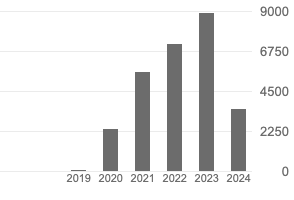
\includegraphics[width=0.5\textwidth]{citation-graph}
\end{minipage}
\end{tabular}



\begin{flushright}\vspace{-5pt}{\footnotesize \it According to Google Scholar on 28th of April, 2024:
  \href{https://scholar.google.com.br/citations?user=5t_sZdMAAAAJ}{\texttt{scholar.google.com.br/citations?user=5t\_sZdMAAAAJ}}}
\end{flushright}



\end{document}

